\documentclass{article}
\usepackage{mathrsfs}
\usepackage{amsmath}
\usepackage{amsthm}
\usepackage{amssymb}
\usepackage{graphicx}
\usepackage{color}
\usepackage{algorithm}
\usepackage{algorithmic}
\usepackage{hyperref}

\theoremstyle{definition}
\newtheorem{theorem}{Theorem}[section]
\newtheorem{lemma}[theorem]{Lemma}
\newtheorem{proposition}[theorem]{Proposition}
\newtheorem{corollary}[theorem]{Corollary}

\theoremstyle{definition}
\newtheorem*{definition}{Definition}
\newtheorem*{example}{Example}

\theoremstyle{remark}
\newtheorem*{remark}{Remark}
\newtheorem*{note}{Note}
\newtheorem*{exercise}{Exercise}

\setlength{\oddsidemargin}{-0.25 in}
\setlength{\evensidemargin}{-0.25 in}
\setlength{\topmargin}{-0.25 in}
\setlength{\textwidth}{7 in}
\setlength{\textheight}{8.5 in}
\setlength{\headsep}{0.25 in}
\setlength{\parindent}{0 in}
\setlength{\parskip}{0.1 in}

\newcommand{\homework}[5]{
\pagestyle{myheadings} \thispagestyle{plain}
\newpage
\setcounter{page}{1} \setcounter{section}{#5} \noindent
\begin{center}
\framebox{ \vbox{\vspace{2mm} \hbox to 6.28in { {\bf
THU-70250043-0,~Pattern~Recognition~(Spring 2021) \hfill Homework: 5} }
\vspace{6mm} \hbox to 6.28in { {\Large \hfill #1 \hfill} }
\vspace{6mm} \hbox to 6.28in { {\it Lecturer: #2 \hfill} }
\vspace{2mm} \hbox to 6.28in { {\it \hspace{15mm} #3 \hfill} }
\vspace{2mm} \hbox to 6.28in { {\it Student: #4 \hfill} }
\vspace{2mm} } }
\end{center}
\markboth{#1}{#1} \vspace*{4mm} }

\begin{document}

\homework{SVM}{Changshui Zhang
\hspace{5mm} {\tt zcs@mail.tsinghua.edu.cn}}{Hong Zhao
\hspace{15mm} {\tt vzhao@tsinghua.edu.cn}}{ \hspace{5mm} {\tt
xxx@mails.tsinghua.edu.cn} }{0}


\section*{Problem 1}
Given an unlabeled set of examples $\left\{x^{(1)},...,x^{(n)} \right\} $ the one-class SVM algorithm tries to find a direction $\omega$ that maximally separates the data from the origin.(This turns out to be useful for anomaly detection.)

More precisely, it solves the (primal) optimization problem:

\begin{equation*}
 \begin{aligned}
 & \min_\omega
 & & \frac{1}{2}\omega^T\omega \\
 & \mbox{s.t.}
 & & \omega^Tx^{(i)}\ge1,
 &
 & & i = 1,\ldots,n
 \end{aligned}
\end{equation*}

A new test example $x$ is labeled 1 if $\omega^Tx\ge1$, and 0 otherwise

1.1 The primal optimization problem for the one-class SVM was given above. Write down the corresponding dual optimization problem. Simplify your answer as much as possible. In particular, $\omega$ should not appear in your answer.

1.2 Can the one-class SVM be kernelized (both in training and testing)? Justify your answer.


\section*{Problem 2}

Consider a dataset with 2 points in 1d: $x_1 = 0$, $x_2 = \sqrt{2}$ with labels $ y_1 = -1$, $y_2 = 1$. Consider mapping each point to 3d using the feature vector $\Phi = [1, \sqrt{2}x, x^2]^T$. (This is equivalent to using a second order polynomial kernel.) The max margin classifier has the form:

\begin{eqnarray}
min ||w||^2   &s.t.& \\
y_1(w^T \Phi(x_1) + b) &\geq &  1  \\
y_2(w^T \Phi(x_2) + b) &\geq &  1  
\end{eqnarray}

a. Write down a vector that is parallel to the optimal vector $w$. 

b. What is the value of the margin that is achieved by this $w$? Hint: recall that the margin is the distance from each support vector to the decision boundary. Hint 2: think about the geometry of 2 points in space, with a line separating one from the other.

c. Solve for $w$, using the fact the margin is equal to $1/||w||$.

d. Write down the form of the discriminant function $ f(x) = w^T\Phi(x) + b$ as an explicit function of $x$.


\section*{Problem 3}
The exclusive-OR is the simplest problem that cannot be solved using a linear discriminant operating directly on the features. The points $k=1,3$ at $\bf{x}=(1,1)^t$ and $\bf{x}=(-1,-1)^t$ are in category $\omega_1$ (red in Figure~\ref{fig:xor}), while $k=2,4$ at $\bf{x}=(1,-1)^t$ and $\bf{x}=(-1,1)^t$ are in $\omega_2$ (black in Figure~\ref{fig:xor}). Following the approach of SVM, we use kernel function to map the features to a higher dimension space where they can be linearly separated.

\begin{figure}[htbp]
    \centering
    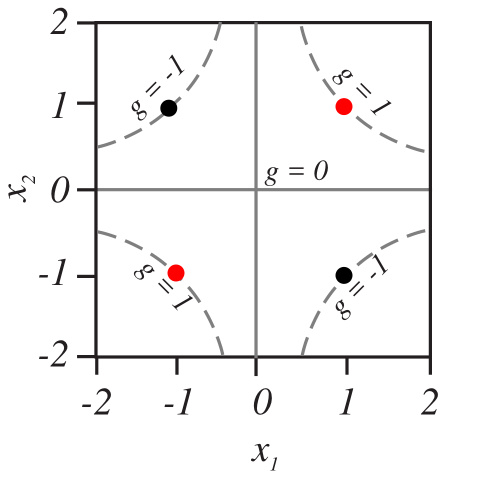
\includegraphics[width=0.3\linewidth]{XOR.PNG}
    \caption{The XOR problem in the original $(x_1,x_2)$ feature space.}
    \label{fig:xor}
\end{figure}

3.1 Consider the polynomial kernel of degree 2: 
\[K(\bf{x_i}, \bf{x_j}) = (\bf{x_i}^t\bf{x_j} + 1)^2,\] where $\boldsymbol{x_i} = (x_{i1}, x_{i2})^t$ and $\boldsymbol{x_j} = (x_{j1}, x_{j2})^t$.

Show that it corresponds to mapping 
\[\Phi(x_1, x_2) = [1, \sqrt{2}x_1, \sqrt{2}x_2, \sqrt{2}x_1x_2, x_1^2, x_2^2].\]

3.2 Derive the dual problem in the 6-dimensional space with Lagrange multipliers $\alpha_i, i=1,2,3,4$ as the only variants.

3.3 Solve the dual problem analytically (without programming). What are the support vectors? \emph{Hint: use the symmetry of the problem.}

3.4 Derive the final discriminant function $g(\bf{x})$ and the decision hyperplane.

3.5 Plot the data points on the subspace of $(\sqrt{2}x_1, \sqrt{2}x_1x_2)$. Demonstrate the decision hyperplane and the margin in your plot.


\section*{Problem 4}

\begin{table}[!ht]
	\centering
	\begin{tabular}{|c|c|c|}
		\hline
		Category & $x_1$ & $x_2$\\
		\hline
		$\omega_1$ & -3.0 & -2.9\\
		$\omega_1$ & 0.5 & 8.7\\
		$\omega_1$ & 2.9 & 2.1\\
		$\omega_1$ & -0.1 & 5.2\\
		$\omega_1$ & -4.0 & 2.2\\
		$\omega_1$ & -1.3 & 3.7\\
		$\omega_1$ & -3.4 & 6.2\\
		$\omega_1$ & -4.1 & 3.4\\
		$\omega_1$ & -5.1 & 1.6\\
		$\omega_1$ & 1.9 & 5.1\\
		\hline
		$\omega_2$ & -2.0 & -8.4\\
		$\omega_2$ & -8.9 & 0.2\\
		$\omega_2$ & -4.2 & -7.7\\
		$\omega_2$ & -8.5 & -3.2\\
		$\omega_2$ & -6.7 & -4.0\\
		$\omega_2$ & -0.5 & -9.2\\
		$\omega_2$ & -5.3 & -6.7\\
		$\omega_2$ & -8.7 & -6.4\\
		$\omega_2$ & -7.1 & -9.7\\
		$\omega_2$ & -8.0 & -6.3\\
		\hline
	\end{tabular}
\end{table}

Write a program to complete the following task adopting the SVM algorithm (you could use some toolkits or source code). Train a SVM classifier with data from $\omega_1$ and $\omega_2$ in the following table. Preprocess each training pattern to form a new vector having components $1,x_1,x_2,x_1^2,x_1x_2$ and $ x_2^2$.

4.1 Train you classifier with just the first point in the $\omega_1$ and $\omega_2$ and find the separating hyperplane and the margin.

4.2 Repeat 4.1 with the first two points in each category (four points total), the first three point and so on, until the transformed patterns cannot be linearly separated in the transformed space.

Hint: You needn't program the SVM algorithm by yourself, you can just use some toolkits or source code such as libsvm \url{http://www.csie.ntu.edu.tw/~cjlin/libsvm/} for MATLAB or scikit-learn \url{https://scikit-learn.org/stable/modules/svm.html#svm-classification} for python. You should declare the toolkit you used in your project.

\end{document}
